\documentclass{article}
\usepackage{iclr2026_conference,times}
\usepackage{iftex}
\ifPDFTeX
\usepackage[T1]{fontenc}
\else
\usepackage{fontspec}
\setmainfont{texgyretermes-regular.otf}[BoldFont=texgyretermes-bold.otf,ItalicFont=texgyretermes-italic.otf,BoldItalicFont=texgyretermes-bolditalic.otf]
\setsansfont{texgyreheros-regular.otf}[BoldFont=texgyreheros-bold.otf,ItalicFont=texgyreheros-italic.otf,BoldItalicFont=texgyreheros-bolditalic.otf]
\setmonofont{texgyrecursor-regular.otf}
\fi
\usepackage{amsmath,amssymb,booktabs,array,graphicx,float}
\usepackage{tikz}
\usetikzlibrary{arrows.meta,positioning}
\usepackage{xcolor}
\definecolor{reportblue}{RGB}{36,75,117}
\usepackage[colorlinks=true,linkcolor=reportblue,citecolor=reportblue,urlcolor=reportblue,breaklinks=true]{hyperref}
\usepackage{xurl}
\urlstyle{same}
\iclrfinalcopy
\newlength{\tablewidth}
% Editable vector styles; no raster paper artwork.
\definecolor{audiocolor}{RGB}{222,236,249}
\definecolor{mindcolor}{RGB}{255,234,204}
\definecolor{statecolor}{RGB}{232,226,246}
\definecolor{voicecolor}{RGB}{226,242,225}
\tikzset{
  arch/.style={x=1cm,y=1cm,font=\small,>=Latex},
  block/.style={draw=reportblue!75,rounded corners=2pt,align=center,inner sep=4pt,minimum height=0.68cm},
  audio/.style={block,fill=audiocolor},
  model/.style={block,fill=statecolor},
  mind/.style={block,fill=mindcolor},
  voice/.style={block,fill=voicecolor},
  note/.style={font=\footnotesize,align=center},
  flow/.style={->,thick,draw=reportblue!85},
  feedback/.style={flow,dashed},
}

% Generated by scripts/make_table_reported_performance.py; edit research/reported-performance.json.
\newcommand{\srqaQCThreshold}{0.75}
\newcommand{\srqaDPODelays}{12.0 / 13.2 / 12.9 / 18.2 / 48.6}

\title{Full-Duplex Speech Reasoning: Architectures and Synchronization}
\author{AI2AI Duplex Project: 20-minute discussion brief}
\hypersetup{pdftitle={Full-Duplex Speech Reasoning: 20-minute Discussion Brief},pdfauthor={AI2AI Duplex Project},pdfsubject={Figure-led literature review; revised 1 October 2026}}

\begin{document}
\maketitle
\lhead{AI2AI Duplex: discussion brief, 1 October 2026}
\rhead{}
\cfoot{\thepage}
\raggedbottom
\setlength{\intextsep}{3pt plus 1pt minus 1pt}
\label{page:mapone}

\section{Architecture map I: parallel codec streams vs. a text backbone}
\begin{figure}[H]
\centering
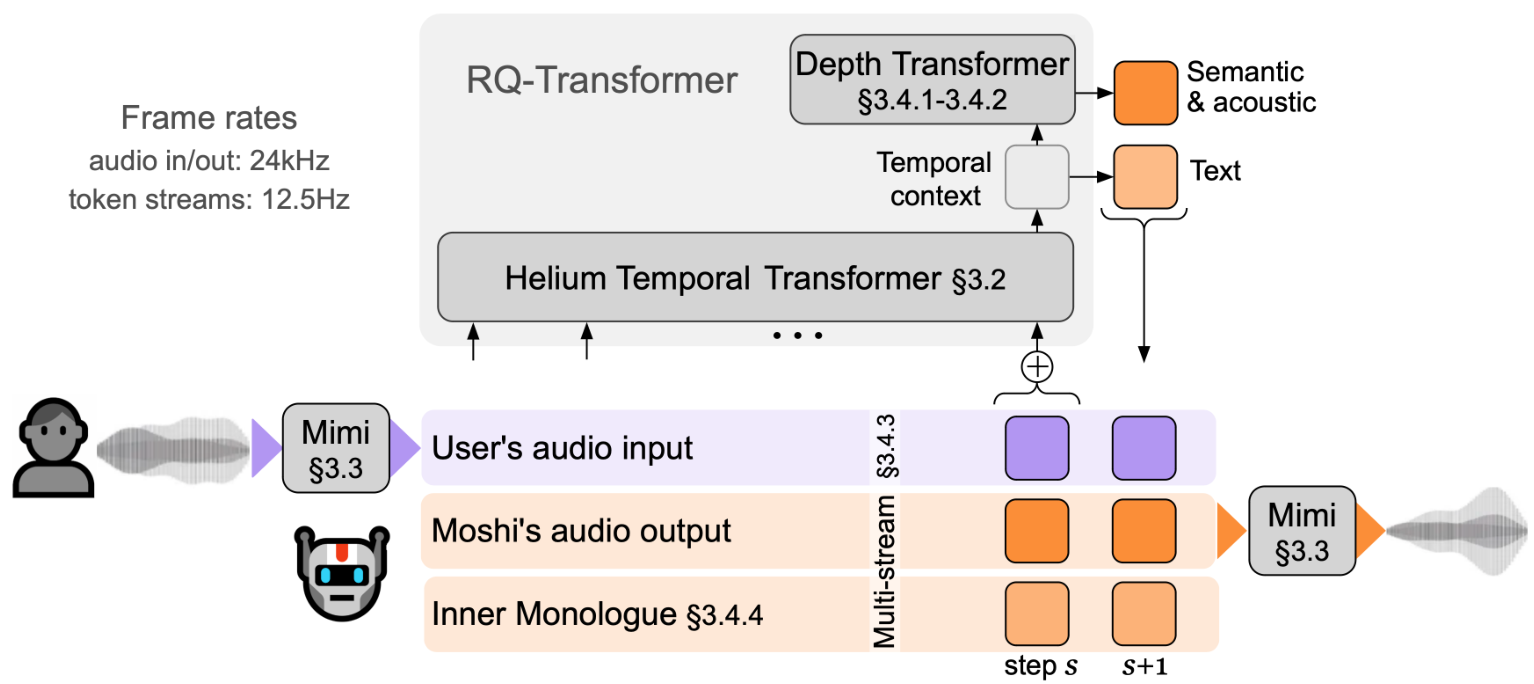
\includegraphics[width=\linewidth]{figures/papers/moshi.png}
\caption{\textbf{Moshi.} Reproduced from \citet{moshi}, Fig.~1. TWL builds on this architecture, adding silent reasoning to the text stream \citep{thinklisten}; that extension is not shown here.}
\label{fig:moshi}
\end{figure}

\begin{figure}[H]
\centering
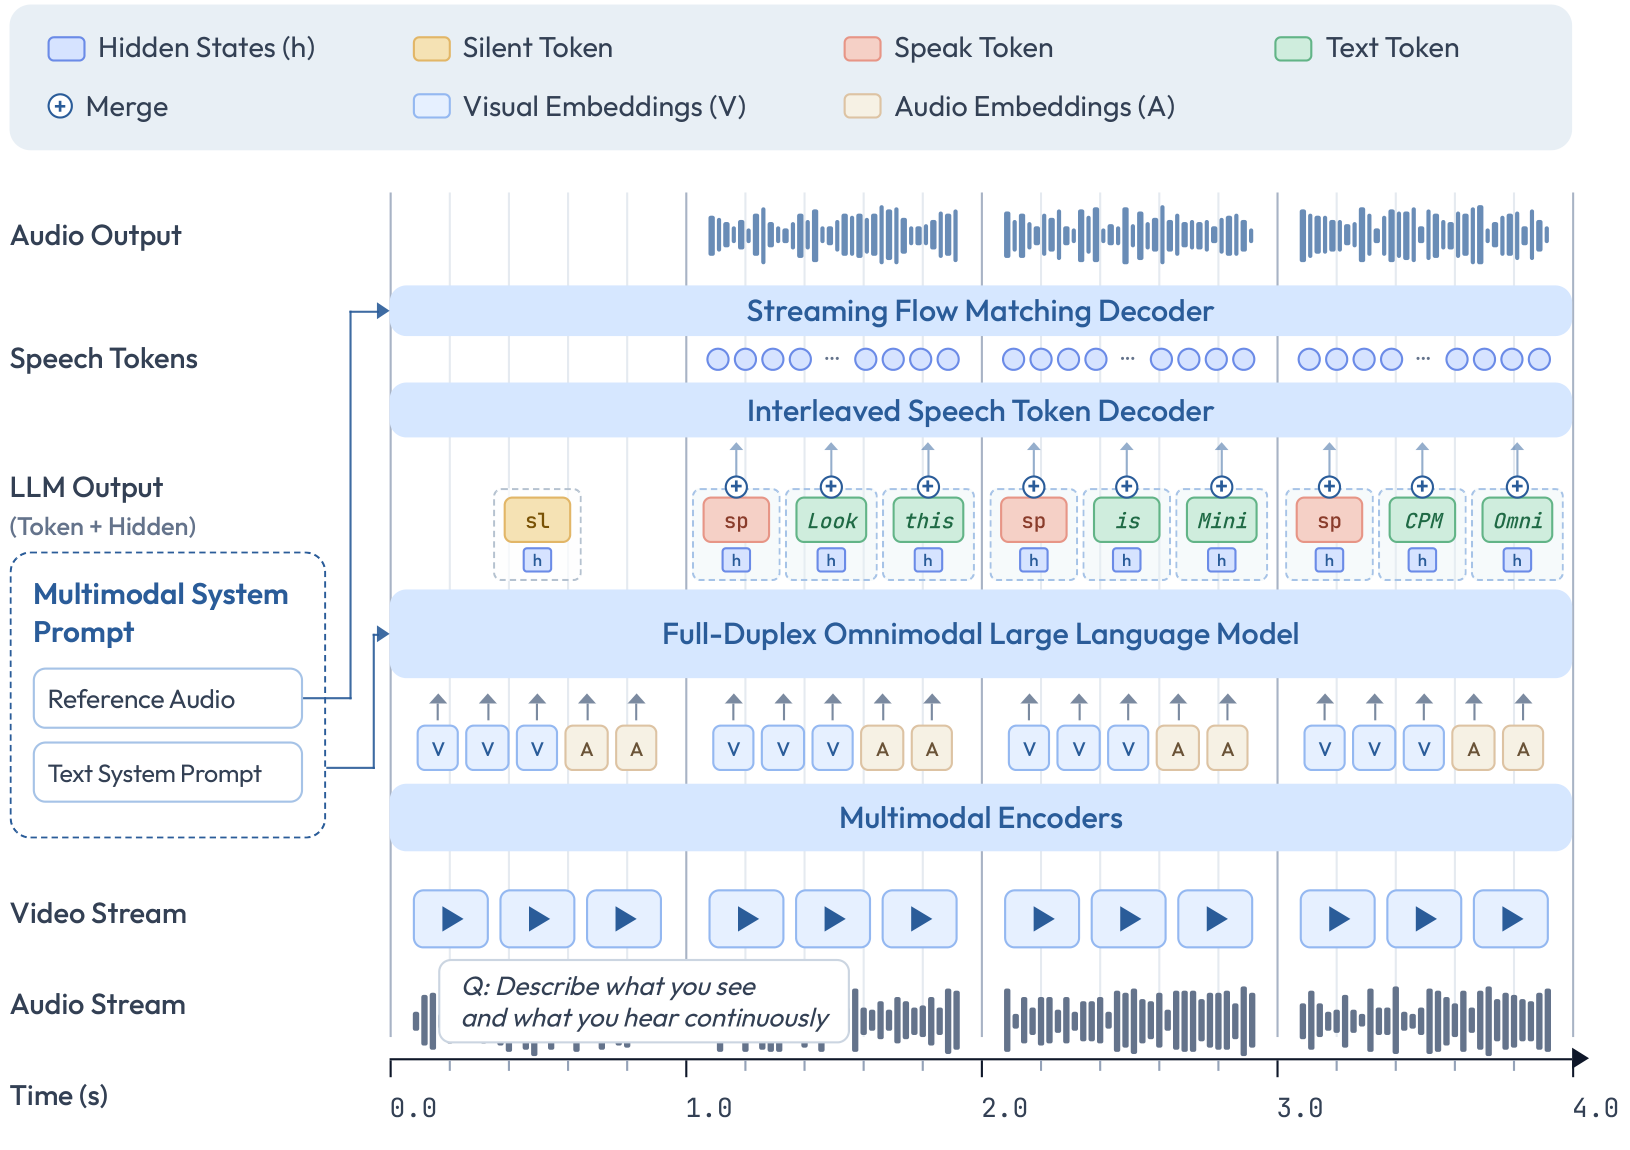
\includegraphics[width=0.94\linewidth]{figures/papers/minicpm.png}
\caption{\textbf{MiniCPM-o 4.5.} Reproduced from \citet{minicpm}, Fig.~4. Timed Qwen3-8B text backbone; separate speech-token and waveform decoders.}
\label{fig:minicpm}
\end{figure}

\newpage
\label{page:maptwo}
\section{Architecture map II: where computation lives}

\begin{figure}[H]
\centering
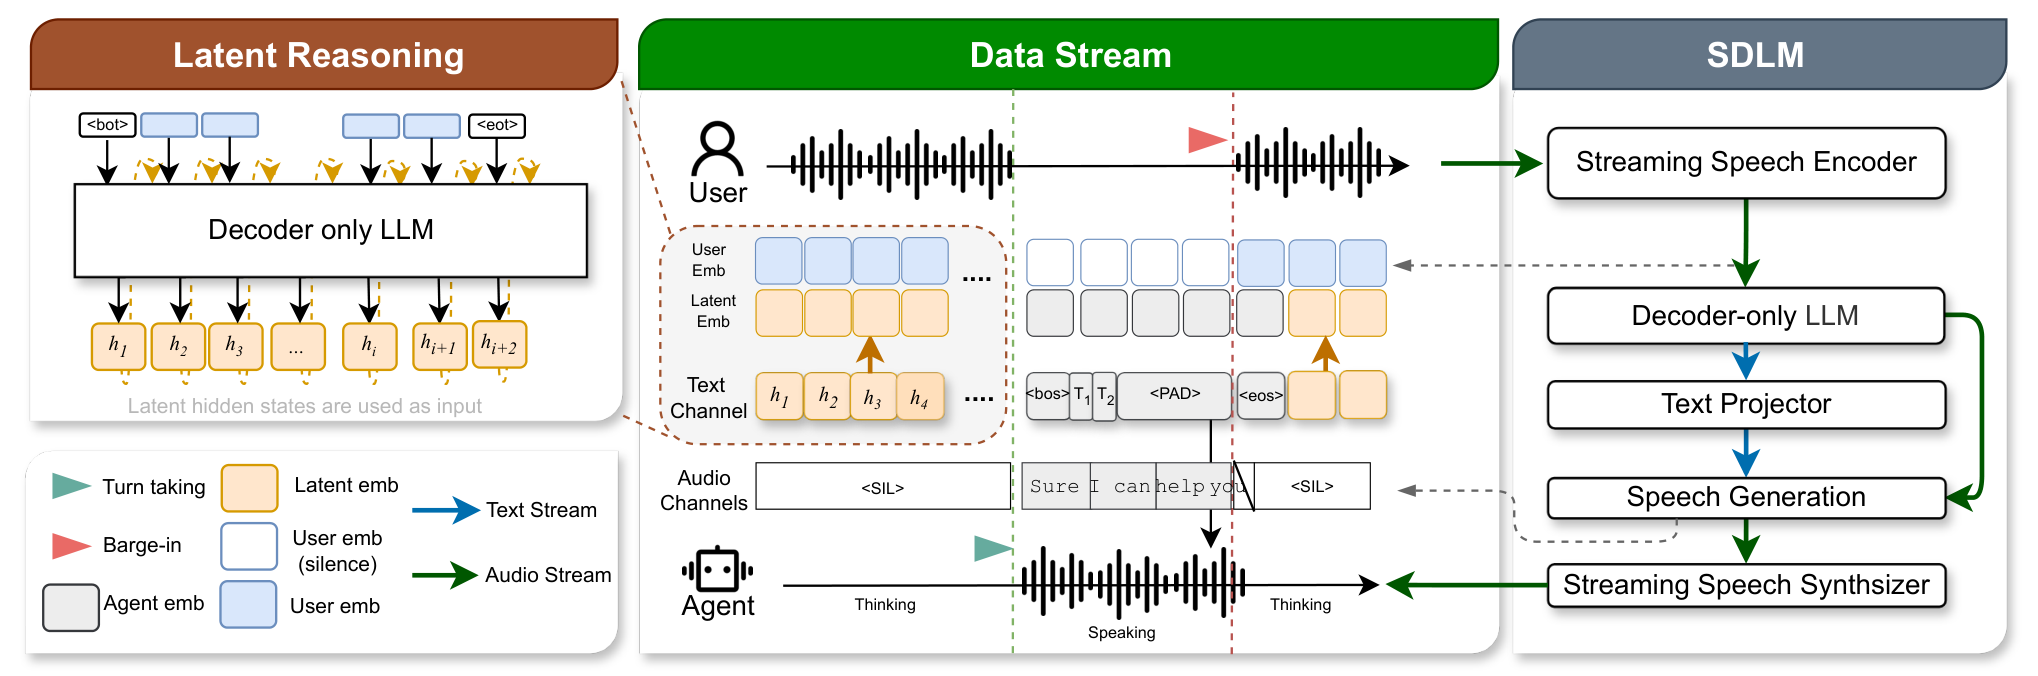
\includegraphics[width=\linewidth]{figures/papers/flair.png}
\caption{\textbf{FLAIR.} Reproduced from \citet{flair}, Fig.~2. Qwen2.5-7B: latent reasoning while listening; text while speaking. Full-context teacher is training-only.}
\label{fig:flair}
\end{figure}

\begin{figure}[H]
\centering
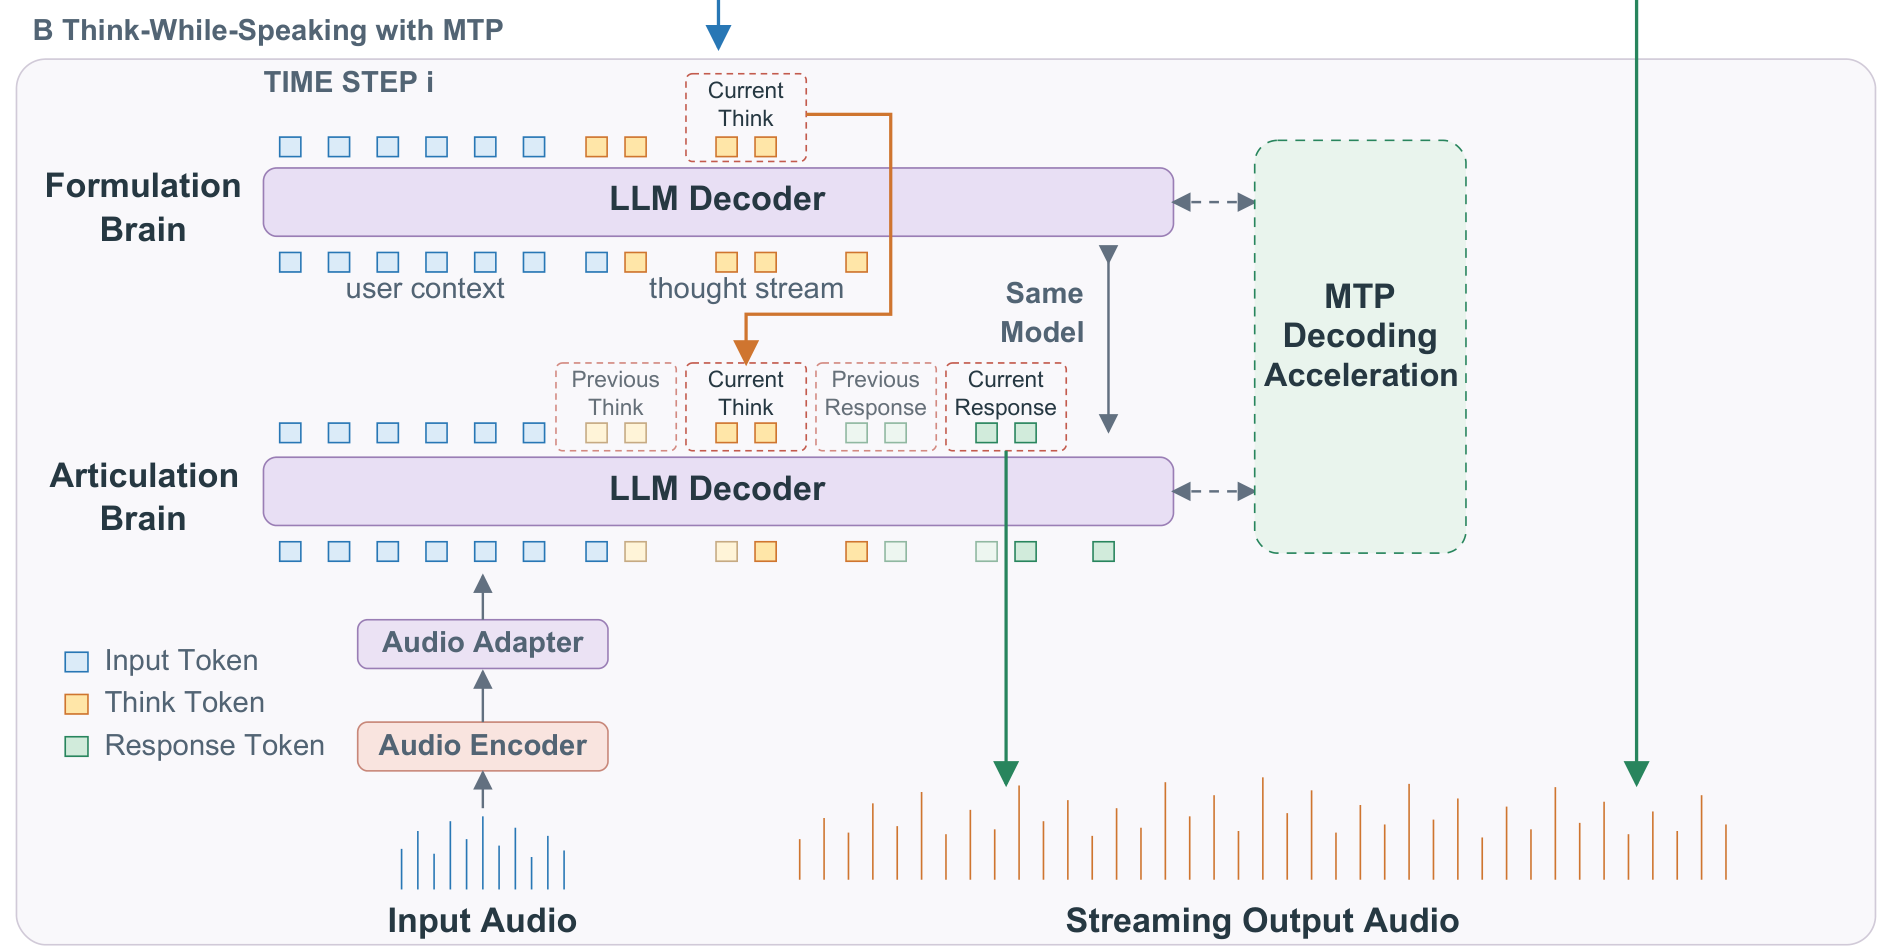
\includegraphics[width=0.85\linewidth]{figures/papers/step3.png}
\caption{\textbf{StepAudio 3 Realtime.} Reproduced from \citet{step3}, Fig.~7B (routing panel A omitted). Same-model formulation/articulation; playback-aware pacing follows Mind-Paced Speaking \citep{mindpaced}.}
\label{fig:step3}
\end{figure}

\begin{figure}[H]
\centering
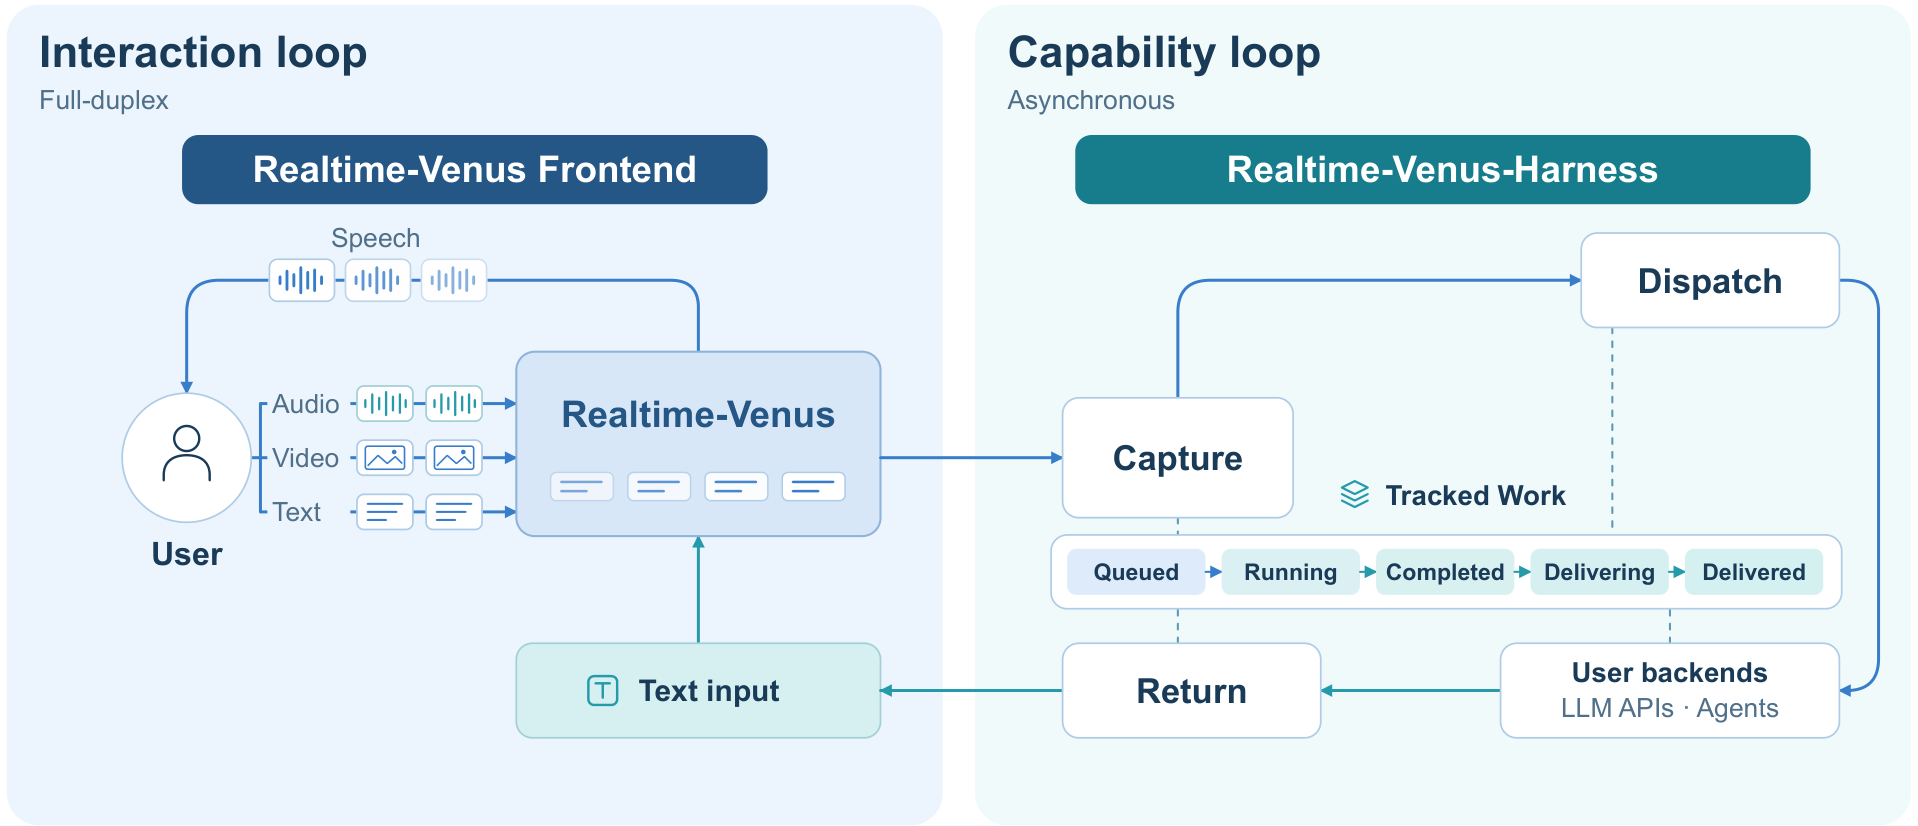
\includegraphics[width=\linewidth]{figures/papers/venus.png}
\caption{\textbf{Realtime-Venus.} Reproduced from \citet{venus}, Fig.~3. Foreground interaction continues during asynchronous delegation; the frontend controls reply delivery timing.}
\label{fig:venus}
\end{figure}

\newpage
\label{page:questions}
\section{Synchronization: incoming speech vs. played speech}

The original proposal centers on \emph{prefix sufficiency, correction-aware reasoning and speaker ownership}. \textbf{Listening sync:} track how much of each speaker's speech the model has \emph{actually processed}, not just received. \textbf{Speaking sync:} distinguish generated speech, buffered audio and speech \emph{already played}. Autoregressive steps are not wall-clock seconds. Wrong claims already played need a spoken correction; buffered audio can still be changed.

\begin{figure}[H]
\centering
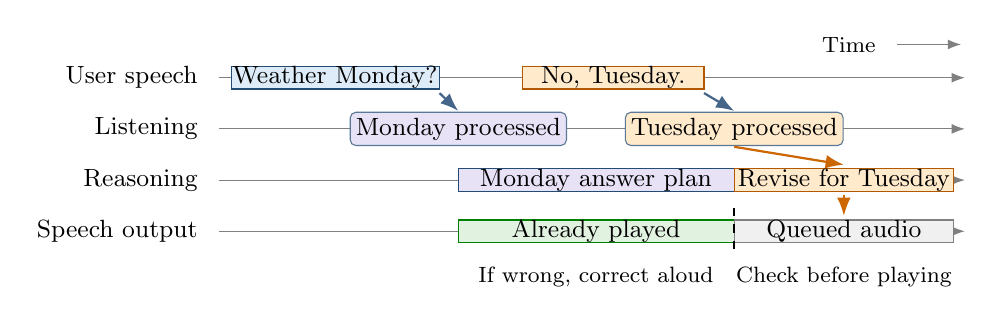
\begin{tikzpicture}[arch,x=0.96cm,y=0.65cm]
\foreach \y/\label in {3/User speech,2/Listening,1/Reasoning,0/Speech output} {
  \node[anchor=east] at (2.13,\y) {\label};
  \draw[->,gray] (2.28,\y)--(12.15,\y);
}
\draw[fill=audiocolor,draw=reportblue] (2.45,2.78) rectangle (5.20,3.22);
\node at (3.82,3) {Weather Monday?};
\draw[fill=mindcolor,draw=orange!70!black] (6.30,2.78) rectangle (8.70,3.22);
\node at (7.50,3) {No, Tuesday.};
\node[model,minimum height=0.40cm,inner sep=2pt] at (5.45,2) {Monday processed};
\node[mind,minimum height=0.40cm,inner sep=2pt] at (9.10,2) {Tuesday processed};
\draw[flow] (5.20,2.7)--(5.45,2.35);
\draw[flow] (8.70,2.7)--(9.10,2.35);
\draw[fill=statecolor,draw=reportblue] (5.45,0.78) rectangle (9.10,1.22);
\node at (7.27,1) {Monday answer plan};
\draw[fill=mindcolor,draw=orange!70!black] (9.10,0.78) rectangle (12.00,1.22);
\node at (10.55,1) {Revise for Tuesday};
\draw[->,orange!80!black,thick] (9.10,1.65)--(10.55,1.30);
\draw[fill=voicecolor,draw=green!50!black] (5.45,-0.22) rectangle (9.10,0.22);
\node at (7.27,0) {Already played};
\draw[fill=gray!12,draw=gray] (9.10,-0.22) rectangle (12.00,0.22);
\node at (10.55,0) {Queued audio};
\draw[->,orange!80!black,thick] (10.55,0.70)--(10.55,0.30);
\draw[dashed,thick] (9.10,-0.35)--(9.10,0.50);
\node[note,anchor=north,text width=3.4cm] at (7.27,-0.50) {If wrong, correct aloud};
\node[note,anchor=north,text width=2.9cm] at (10.55,-0.50) {Check before playing};
\node[note,anchor=east] at (11.10,3.65) {Time};
\draw[->,gray] (11.25,3.65)--(12.10,3.65);
\end{tikzpicture}

\caption{\textbf{Illustrative example, not an experiment.} User speech enters as streaming audio tokens or features, depending on the model. Once the Tuesday correction is processed, revise the answer plan and check buffered audio before playback. A wrong claim already played cannot be taken back; correct it aloud.}
\label{fig:commitment}
\end{figure}

% Generated by scripts/generate_brief.py; edit research/brief_data.py.
\begin{table}[H]
\centering\small
\setlength{\tabcolsep}{4pt}
\setlength{\tablewidth}{\dimexpr\linewidth-2\tabcolsep\relax}
\renewcommand{\arraystretch}{1.06}
\caption{Five closest synchronization references: what already exists.}
\label{tab:synchronization}
\begin{tabular}{@{}>{\raggedright\arraybackslash}p{0.38\tablewidth}>{\raggedright\arraybackslash}p{0.62\tablewidth}@{}}
\toprule
\textbf{Paper} & \textbf{Established mechanism} \\
\midrule
\textbf{SyncLLM} \citep{syncllm} & Clock-aligned chunks; speculative user tokens replaced by observations. \\
\addlinespace[2pt]
\textbf{Moshi} \citep{moshi} & Parallel user/agent codec streams on an 80 ms frame grid. \\
\addlinespace[2pt]
\textbf{DuplexSLA} \citep{duplexsla} & 160 ms speech/listening/action clock; release marked forthcoming. \\
\addlinespace[2pt]
\textbf{AdaptDuplex} \citep{adapt} & Adaptive windows, bounded text lead, cancel / stale-result suppression. \\
\addlinespace[2pt]
\textbf{Synchronization / turn-taking} \citep{synchrony} & Moshi--Moshi hidden-state coupling and causal timing probes, not reasoning correctness. \\
\bottomrule
\end{tabular}
\end{table}

% Generated by scripts/generate_brief.py; edit research/brief_data.py.
\begin{table}[H]
\centering\small
\setlength{\tabcolsep}{4pt}
\setlength{\tablewidth}{\dimexpr\linewidth-4\tabcolsep\relax}
\renewcommand{\arraystretch}{1.06}
\caption{Five discussion questions: small falsifiable tests, not claimed results.}
\label{tab:questions}
\begin{tabular}{@{}>{\raggedright\arraybackslash}p{0.32\tablewidth}>{\raggedright\arraybackslash}p{0.43\tablewidth}>{\raggedright\arraybackslash}p{0.25\tablewidth}@{}}
\toprule
\textbf{Question} & \textbf{First paired test} & \textbf{Measure} \\
\midrule
\textbf{RQ1: Think while listening}\par When is a prefix sufficient? & Late constraints with identical prefixes; risk-calibrated vs. fixed triggers. & Correct useful-answer time; premature claims. \\
\addlinespace[2pt]
\textbf{RQ2: Think while speaking}\par How much speech lead is safe? & Corrections before / after playback; bounded vs. unrestricted queue. & Stale audible seconds; repair; underruns. \\
\addlinespace[2pt]
\textbf{RQ3: Listen while speaking}\par Whose correction updates what? & Relevant correction vs. backchannel / side speech; oracle vs. predicted identity. & Correction accuracy; false interruption; silence. \\
\addlinespace[2pt]
\textbf{RQ4: Synchronize the clocks}\par Which schedule survives load? & Same audio under rate / jitter / contention; fixed vs. adaptive quantum. & p95 evidence age; useful-answer delay; quality. \\
\addlinespace[2pt]
\textbf{RQ5: Revise while delegating}\par Which returned answer is valid? & Correction during a simulated backend job; cancellation vs. joint result / playback validation. & Stale-result use; task success; wasted work. \\
\bottomrule
\end{tabular}
\end{table}


\textbf{Novelty boundary.} Early thought, dual-process articulation, adaptive windows and stale-job suppression already exist \citep{thinklisten,mindpaced,adapt}. The candidate contribution is \emph{joint speaker/evidence/playback consistency}, tested against those mechanisms. Five questions are discussion options, not ranked winners.

\newpage
\label{page:resources}
\section{Resource sheet and a small first test}
% Generated by scripts/generate_brief.py; edit research/brief_data.py.
\begin{table}[H]
\centering\small
\setlength{\tabcolsep}{4pt}
\setlength{\tablewidth}{\dimexpr\linewidth-4\tabcolsep\relax}
\renewcommand{\arraystretch}{1.06}
\caption{Five evaluation choices: complementary, not one leaderboard.}
\label{tab:benchmarks}
\begin{tabular}{@{}>{\raggedright\arraybackslash}p{0.25\tablewidth}>{\raggedright\arraybackslash}p{0.34\tablewidth}>{\raggedright\arraybackslash}p{0.41\tablewidth}@{}}
\toprule
\textbf{Benchmark} & \textbf{What it tests} & \textbf{Access / interpretation} \\
\midrule
\textbf{SRQA} \citep{thinklisten} & Streaming reasoning accuracy vs. post-question CoT delay. & Synthetic; recipe verified, released evaluation not located. CoT onset is not a useful answer. \\
\addlinespace[2pt]
\textbf{$\tau$-Voice} \citep{tauvoice} & Grounded tool/task success across 278 tasks. & Code / tasks / simulator; APIs needed. Virtual time is not physical deadline validation. \\
\addlinespace[2pt]
\textbf{Full-Duplex-Bench v3} \citep{fdb3} & Human disfluencies, tools, argument accuracy and completion. & Code + recordings. Tool F1 does not equal task success. \\
\addlinespace[2pt]
\textbf{EchoChain} \citep{echochain} & State revision during speech: inertia, amnesia, goal loss. & 200 synthetic interrupted conversations; standalone release not located. \\
\addlinespace[2pt]
\textbf{Duplex-MPE} \citep{mpe} & Addressee control, silence, answers and floor release. & 4,000 synthetic streams; standalone release not located. \\
\bottomrule
\end{tabular}
\end{table}

% Generated by scripts/generate_brief.py; edit research/brief_data.py.
\begin{table}[H]
\centering\small
\setlength{\tabcolsep}{4pt}
\setlength{\tablewidth}{\dimexpr\linewidth-4\tabcolsep\relax}
\renewcommand{\arraystretch}{1.06}
\caption{Five supervision sources: natural timing is not a reasoning label.}
\label{tab:data}
\begin{tabular}{@{}>{\raggedright\arraybackslash}p{0.25\tablewidth}>{\raggedright\arraybackslash}p{0.38\tablewidth}>{\raggedright\arraybackslash}p{0.37\tablewidth}@{}}
\toprule
\textbf{Resource} & \textbf{Useful content / scale} & \textbf{Access / caution} \\
\midrule
\textbf{SmoothConv} \citep{smoothconv} & 100.53 h Chinese; speaker / turn-state / timing labels. & HF; CC BY-NC 4.0; shared sources with DuplexConv. \\
\addlinespace[2pt]
\textbf{DuplexConv} \citep{duplexconv} & 2,000.21 h Chinese; channels, VAD and machine-assisted labels. & HF; CC BY-NC 4.0; split by source session. \\
\addlinespace[2pt]
\textbf{otoSpeech Task} \citep{ototask} & 20.006 h / 58 English sessions; channels and task events. & Gated; CC BY 4.0; verify task-outcome labels. \\
\addlinespace[2pt]
\textbf{otoSpeech conversational} \citep{otoconv} & 280 h raw / 141 h curated English; separate speaker channels. & Gated; CC BY 4.0; curated data is a subset. \\
\addlinespace[2pt]
\textbf{Open Yap 1K} \citep{openyap} & 1,000 h English; word timing, familiar-speaker dyads. & Public sample; full corpus requires request / DUA. \\
\bottomrule
\end{tabular}
\end{table}


\begin{figure}[H]
\centering
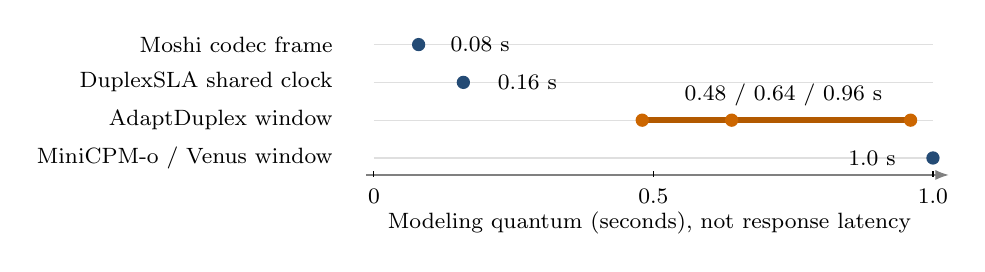
\begin{tikzpicture}[arch,x=1cm,y=0.48cm]
\draw[->,gray] (4.85,-0.45)--(12.25,-0.45);
\foreach \v/\label in {0/0,0.5/0.5,1/1.0} {
  \draw (4.95+7.1*\v,-0.50)--(4.95+7.1*\v,-0.34);
  \node[note,anchor=north] at (4.95+7.1*\v,-0.56) {\label};
}
\node[note,anchor=east] at (4.55,3) {Moshi codec frame};
\node[note,anchor=east] at (4.55,2) {DuplexSLA shared clock};
\node[note,anchor=east] at (4.55,1) {AdaptDuplex window};
\node[note,anchor=east] at (4.55,0) {MiniCPM-o / Venus window};
\foreach \y in {0,1,2,3} {\draw[gray!25] (4.95,\y)--(12.05,\y);}
\fill[reportblue] (4.95+7.1*0.08,3) circle (2.4pt);
\node[note,anchor=west] at (5.80,3) {0.08 s};
\fill[reportblue] (4.95+7.1*0.16,2) circle (2.4pt);
\node[note,anchor=west] at (6.40,2) {0.16 s};
\draw[line width=2pt,orange!70!black] (4.95+7.1*0.48,1)--(4.95+7.1*0.96,1);
\foreach \v in {0.48,0.64,0.96} {\fill[orange!80!black] (4.95+7.1*\v,1) circle (2.4pt);}
\node[note,anchor=south] at (10.15,1.12) {0.48 / 0.64 / 0.96 s};
\fill[reportblue] (12.05,0) circle (2.4pt);
\node[note,anchor=east] at (11.70,0) {1.0 s};
\node[note,anchor=north] at (8.45,-1.17) {Modeling quantum (seconds), not response latency};
\end{tikzpicture}

\caption{\textbf{Published timing parameters, not a latency leaderboard.} Codec frames, shared action clocks and language windows are different quantities \citep{moshi,duplexsla,adapt,minicpm,venus}. Smaller quantum does not imply a faster \emph{correct} answer.}
\label{fig:timing}
\end{figure}

\textbf{First test.} Instrument a released 7--9B runtime on 200--500 paired dialogues: relevant correction vs. backchannel; before vs. after playback; same vs. different speaker. Keep model, lookahead and compute budget fixed; use a simulated read-only backend. Log ingestion, state version, output queue and playback. Compare \emph{correct useful-answer latency, stale audible seconds, final task success and false interruption}, not first filler sound. Natural corpora need added sufficiency/revision labels; hold out benchmark tests. No experiments or performance measurements were run for this brief.

{\small Literature/availability cutoff: 30 September 2026. “Not located” is not proof of nonexistence. Details and caveats: see the preserved nine-page report and source notes.}

\newpage
\label{page:performance}
\section{Reported performance on the selected benchmarks}
These are source-reported results, not our experiments. Original benchmark comparisons and later system-report evaluations are labeled separately; their model versions, conditions and aggregation can differ.

% Generated by scripts/make_table_reported_performance.py; edit research/reported-performance.json.
\begin{table}[H]
\centering\small
\setlength{\tabcolsep}{4pt}
\setlength{\tablewidth}{\dimexpr\linewidth-4\tabcolsep\relax}
\renewcommand{\arraystretch}{1.06}
\caption{Reported performance (percent, higher is better). Scores follow the metric order in each row; compare only within a protocol. NR: selected-system result not located, not zero. Closed references are the best in the stated source comparison, not a current global leaderboard.}
\label{tab:performance}
\begin{tabular}{@{}>{\raggedright\arraybackslash}p{0.28\tablewidth}>{\raggedright\arraybackslash}p{0.44\tablewidth}>{\raggedright\arraybackslash}p{0.28\tablewidth}@{}}
\toprule
\textbf{Benchmark / metric order} & \textbf{Selected systems} & \textbf{Best closed voice in source} \\
\midrule
\textbf{SRQA}\par ICLR proceedings; ARC-E / ARC-C / SIQA / PIQA / GSM8K\par\citep{thinklisten} & \textbf{Moshi + CoT (TWL study)}\par 77.7 / 59.8 / 56.1 / 56.9 / 16.1\par\smallskip \textbf{TWL: early length-DPO}\par 65.4 / 46.0 / 45.3 / 46.0 / 14.7 & No closed voice result. \\
\addlinespace[2pt]
\textbf{$\tau$-Voice}\par Original benchmark, Table 6 All row; clean / realistic\par\citep{tauvoice} & NR & \textbf{Grok Voice}\par 51 / 38 \\
\addlinespace[2pt]
\textbf{$\tau$-Voice (AA)}\par Artificial Analysis implementation; equal-domain macro task-success rate\par\citep{step3} & \textbf{StepAudio 3 Realtime}\par 56.0 & \textbf{Grok Voice Think Fast 2.0 High}\par 56.5 \\
\addlinespace[2pt]
\textbf{Full-Duplex-Bench v3}\par Tool selection F1 / argument accuracy / pass@1\par\citep{fdb3,venus} & \textbf{Realtime-Venus-Omni}\par 86.0 / 53.1 / 43.0\par\smallskip \textbf{Realtime-Venus-Audio}\par 82.0 / 52.2 / 42.0 & \textbf{GPT-Realtime}\par 87.6 / 68.0 / 60.0 \\
\addlinespace[2pt]
\textbf{EchoChain}\par 200 interrupted conversations; conversation MPR / criterion MCP\par\citep{echochain} & NR & \textbf{Grok Voice Agent}\par 48.5 / 85.5 \\
\addlinespace[2pt]
\textbf{Duplex-MPE}\par Explicit / implicit addressing; fresh onset / conditional answer / silence / yield\par\citep{mpe} & \textbf{MiniCPM-o 4.5 (explicit)}\par 95.00 / 47.30 / 92.42 / 59.64\par\smallskip \textbf{MiniCPM-o 4.5 (implicit)}\par 94.35 / 46.65 / 92.89 / 59.25 & No closed voice result. \\
\bottomrule
\end{tabular}
\end{table}

\smallskip
{\small\textbf{Text controls, not voice competitors.} Original $\tau$-Voice: GPT-5 reasoning, 85\% task pass@1. Duplex-MPE: Gemini 3.1 Pro with speaker-attributed transcripts, explicit 94.70 / 90.39 / 95.37, implicit 30.40 / 79.11 / 99.34 (response presence / conditional answer / silence, \%; Table 17 reference run). No fresh-onset or stopping score; not a speech-model upper bound. \citep{tauvoice,mpe}}


{\small\textbf{Coverage and configuration caveats.} FLAIR has no located score on these five benchmarks; its Full-Duplex-Bench results use an earlier version. SRQA's CoT and early-DPO rows are different checkpoints (Tables 2 and 4); early-DPO uses question-completeness threshold \srqaQCThreshold, with delays of \srqaDPODelays{} tokens in the same task order, not runtime seconds. Venus's v3 scores come from its revised report, not a common rerun with the benchmark authors. The two $\tau$-Voice rows are not interchangeable. Duplex-MPE yield has model-specific eligibility; Gemini's text reference supplies speaker identity. Unlisted selected-system/benchmark pairs are NR.}

\smallskip
\textbf{Reading the gaps.} Tool selection can be strong while complete-task success remains weak; a response can occur without being correct or appropriate. The missing cross-system coverage is itself a reason to build a shared, version-pinned evaluation harness, not evidence that an untested system fails.

\newpage
\label{page:references}
\section*{Availability and references}
% Generated by scripts/generate_brief.py; edit research/brief_data.py.
\begin{table}[H]
\centering\small
\setlength{\tabcolsep}{4pt}
\setlength{\tablewidth}{\dimexpr\linewidth-4\tabcolsep\relax}
\renewcommand{\arraystretch}{1.06}
\caption{Five system anchors: availability snapshot, 30 September 2026.}
\label{tab:systems}
\begin{tabular}{@{}>{\raggedright\arraybackslash}p{0.31\tablewidth}>{\raggedright\arraybackslash}p{0.36\tablewidth}>{\raggedright\arraybackslash}p{0.33\tablewidth}@{}}
\toprule
\textbf{System} & \textbf{Inference / weights} & \textbf{Training reproducibility} \\
\midrule
\textbf{Think while listening} & Study release not located; base Moshi is released. & Recipe; full spoken-CoT data not located. \\
\addlinespace[2pt]
\textbf{FLAIR} & Dedicated code / weights not located. & Latent ELBO/SFT; full mixture not located. \\
\addlinespace[2pt]
\textbf{MiniCPM-o 4.5} & Released code + weights; Apache-2.0. & Fine-tuning tools; complete duplex mixture not released. \\
\addlinespace[2pt]
\textbf{StepAudio 3 Realtime} & Report / demos; Realtime weights not located. & Methods; full code / mixture not located. \\
\addlinespace[2pt]
\textbf{Realtime-Venus} & Released harness + Audio/Omni weights; Apache-2.0. & Methods; complete training package not located. \\
\bottomrule
\end{tabular}
\end{table}

\begingroup
\footnotesize
\setlength{\parskip}{2pt}
% Generated compact linked references; full BibTeX in references.bib.
\begin{thebibliography}{99}
\bibitem[Shih et al.(2026)]{thinklisten}
Shih et al. (2026). \href{https://proceedings.iclr.cc/paper_files/paper/2026/file/75c45fca2aa416ada062b26cc4fb7641-Paper-Conference.pdf}{Can Speech LLMs Think while Listening?}. ICLR 2026.
\bibitem[Wu et al.(2026)]{flair}
Wu et al. (2026). \href{https://arxiv.org/abs/2603.17837}{The Silent Thought: Modeling Internal Cognition in Full-Duplex Spoken Dialogue Models via Latent Reasoning}. Preprint / technical report.
\bibitem[Cui et al.(2026)]{minicpm}
Cui et al. (2026). \href{https://arxiv.org/abs/2604.27393}{MiniCPM-o 4.5: Towards Real-Time Full-Duplex Omni-Modal Interaction}. Preprint / technical report.
\bibitem[Lin et al.(2026a)]{step3}
Lin et al. (2026a). \href{https://arxiv.org/abs/2609.14005}{StepAudio 3 Realtime Technical Report}. Preprint / technical report.
\bibitem[Ant Group(2026)]{venus}
Ant Group (2026). \href{https://arxiv.org/abs/2609.13814}{Realtime-Venus: A full-duplex interaction system with asynchronous delegation}. Preprint / technical report.
\bibitem[Veluri et al.(2024)]{syncllm}
Veluri et al. (2024). \href{https://aclanthology.org/2024.emnlp-main.1192/}{Beyond Turn-Based Interfaces: Synchronous LLMs as Full-Duplex Dialogue Agents}. EMNLP 2024.
\bibitem[Défossez et al.(2024)]{moshi}
Défossez et al. (2024). \href{https://arxiv.org/abs/2410.00037}{Moshi: a speech-text foundation model for real-time dialogue}. Preprint / technical report.
\bibitem[Zhang et al.(2026)]{duplexsla}
Zhang et al. (2026). \href{https://arxiv.org/abs/2605.20755}{DuplexSLA: A Full-Duplex Spoken Language Model with Synchronized Speech, Language, and Action}. Preprint / technical report.
\bibitem[Zhou et al.(2026)]{adapt}
Zhou et al. (2026). \href{https://arxiv.org/abs/2609.29217}{AdaptDuplex: from static to adaptive full-duplex spoken dialogue}. Preprint / technical report.
\bibitem[Riera et al.(2026)]{synchrony}
Riera et al. (2026). \href{https://arxiv.org/abs/2605.20356}{Synchronization and Turn-Taking in Full-Duplex Speech Dialogue Models}. Preprint / technical report.
\bibitem[Ray et al.(2026)]{tauvoice}
Ray et al. (2026). \href{https://proceedings.mlr.press/v306/ray26a.html}{$\tau$-Voice: Benchmarking Full-Duplex Voice Agents on Real-World Domains}. ICML 2026.
\bibitem[Lin et al.(2026b)]{fdb3}
Lin et al. (2026b). \href{https://arxiv.org/abs/2604.04847}{Full-Duplex-Bench-v3: Benchmarking Tool Use for Full-Duplex Voice Agents Under Real-World Disfluency}. Preprint / technical report.
\bibitem[Modi et al.(2026)]{echochain}
Modi et al. (2026). \href{https://arxiv.org/abs/2604.16456}{EchoChain: A Full-Duplex Benchmark for State-Update Reasoning Under Interruptions}. Preprint / technical report.
\bibitem[Ma et al.(2026)]{mpe}
Ma et al. (2026). \href{https://arxiv.org/abs/2609.31948}{Duplex-MPE: Benchmarking Multi-Party Interaction in Full-Duplex Dialogue}. Preprint / technical report.
\bibitem[Wu et al.(2025)]{mindpaced}
Wu et al. (2025). \href{https://arxiv.org/abs/2510.09592}{Mind-Paced Speaking: A Dual-Brain Approach to Real-Time Reasoning in Spoken Language Models}. Preprint / technical report.
\bibitem[QualiaLabs(n.d.)]{smoothconv}
QualiaLabs (n.d.). \href{https://huggingface.co/datasets/qualialabsAI/SmoothConv}{SmoothConv dataset documentation}. Accessed 30 September 2026.
\bibitem[OpenT2S(n.d.)]{duplexconv}
OpenT2S (n.d.). \href{https://huggingface.co/datasets/OpenT2S/DuplexConv}{DuplexConv dataset documentation}. Accessed 30 September 2026.
\bibitem[otoEarth(n.d.-a)]{ototask}
otoEarth (n.d.-a). \href{https://huggingface.co/datasets/otoearth/otoSpeech-full-duplex-task-oriented-20h}{otoSpeech Task dataset documentation}. Accessed 30 September 2026.
\bibitem[otoEarth(n.d.-b)]{otoconv}
otoEarth (n.d.-b). \href{https://huggingface.co/datasets/otoearth/otoSpeech-full-duplex-processed-141h}{otoSpeech conversational dataset documentation}. Accessed 30 September 2026.
\bibitem[The Agentic Data Company(n.d.)]{openyap}
The Agentic Data Company (n.d.). \href{https://github.com/The-Agentic-Data-Co/open-yap-1k}{Open Yap 1K dataset documentation}. Accessed 30 September 2026.
\end{thebibliography}

\endgroup
\end{document}
